\begin{frame}[fragile]{Advanced Figure Techniques: Multiple Figures}
     \textbf{Side-by-side figures using minipage:}
     \begin{lstlisting}
% Side-by-side figures (no subcaption package needed)
\begin{figure}
   \centering
   % First figure
   \begin{minipage}{0.45\textwidth}
        \centering
        \includegraphics[width=\textwidth]{image1}
        \caption{First image}
        \label{fig:img1}
   \end{minipage}
   \hfill
   % Second figure
   \begin{minipage}{0.45\textwidth}
        \centering
        \includegraphics[width=\textwidth]{image2}
        \caption{Second image}
        \label{fig:img2}
   \end{minipage}
\end{figure}
     \end{lstlisting}
\end{frame}

\begin{frame}
	     
	\textbf{Key points:}
	\begin{itemize}
		\item Uses standard \texttt{minipage} environment
		\item Works with base LaTeX, no additional packages needed
		\item Each minipage has its own caption and label
		\item Use \texttt{hfill} for equal spacing
	\end{itemize}
	
	\begin{tip}
		If you need more control, use the \texttt{subcaption} package and add \texttt{\textbackslash usepackage\{subcaption\}} to your preamble
	\end{tip}
\end{frame}
\begin{frame}{Template: Side-by-Side Figures}
     \begin{figure}
          \centering
          % First figure
          \begin{minipage}{0.45\textwidth}
               \centering
               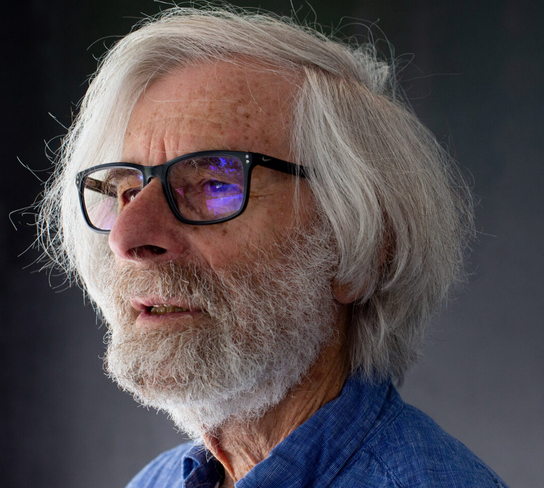
\includegraphics[width=\textwidth]{figs/Lamport.png}
               \caption{Lamport}
               \label{fig:latex_logo}
          \end{minipage}
          \hfill
          % Second figure
          \begin{minipage}{0.45\textwidth}
               \centering
               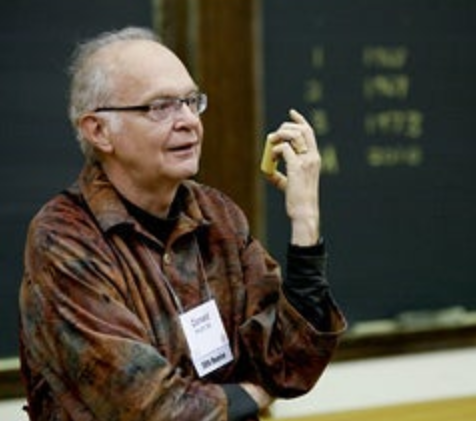
\includegraphics[width=\textwidth]{figs/knuth}
               \caption{Donald Knuth}
               \label{fig:knuth}
          \end{minipage}
     \end{figure}
     
     \begin{itemize}
          \item The figures above show key elements of LaTeX history
          \item Each image has its own caption and reference label
          \item References work normally: Figure~\ref{fig:latex_logo} shows the logo
     \end{itemize}
\end{frame}

\begin{frame}[fragile]{Vertical Figure Arrangements}
     \textbf{Stacked figures with separate captions:}
     \begin{lstlisting}
% Vertical arrangement of two figures
\begin{figure}
   \centering
   \includegraphics[width=0.6\textwidth]{image1}
   \caption{First image}
   \label{fig:img1}
   
   \vspace{1cm}
   
   \includegraphics[width=0.6\textwidth]{image2}
   \caption{Second image}
   \label{fig:img2}
\end{figure}
     \end{lstlisting}
     
     \textbf{Creating a 2×2 grid layout:}
     \begin{lstlisting}
% 2x2 grid using minipages
\begin{figure}
   \centering
   % Top row
   \begin{minipage}{0.45\textwidth}
\centering
        \includegraphics[width=\textwidth]{img1}
        \caption{Top left}
        \label{fig:topleft}
   \end{minipage}
   \hfill
   \begin{minipage}{0.45\textwidth}
        \centering
        \includegraphics[width=\textwidth]{img2}
        \caption{Top right}
        \label{fig:topright}
   \end{minipage}
   
   \vspace{1cm}
   
   % Bottom row
   \begin{minipage}{0.45\textwidth}
        \centering
        \includegraphics[width=\textwidth]{img3}
        \caption{Bottom left}
        \label{fig:bottomleft}
   \end{minipage}
   \hfill
   \begin{minipage}{0.45\textwidth}
        \centering
        \includegraphics[width=\textwidth]{img4}
        \caption{Bottom right}
        \label{fig:bottomright}
   \end{minipage}
\end{figure}
     \end{lstlisting}
\end{frame}
\begin{frame}{Template: 2×2 Grid of Figures}
     \begin{figure}
          \centering
          % Top row
          \begin{minipage}{0.2\textwidth}
               \centering
               
\includegraphics[width=\textwidth]{figs/latex_logo}
               \caption{LaTeX Logo}
               \label{fig:grid_tl}
          \end{minipage}
          \hspace{1cm}  % Fixed spacing instead of \hfill
          \begin{minipage}{0.2\textwidth}
               \centering
               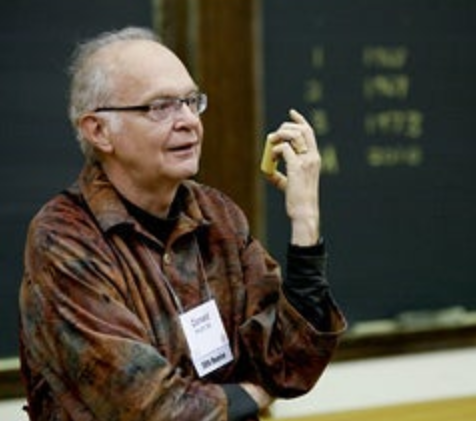
\includegraphics[width=\textwidth]{figs/knuth}
               \caption{Donald Knuth}
               \label{fig:grid_tr}
          \end{minipage}
          
          \vspace{1cm}
          
          % Bottom row
          \begin{minipage}{0.2\textwidth}
               \centering
               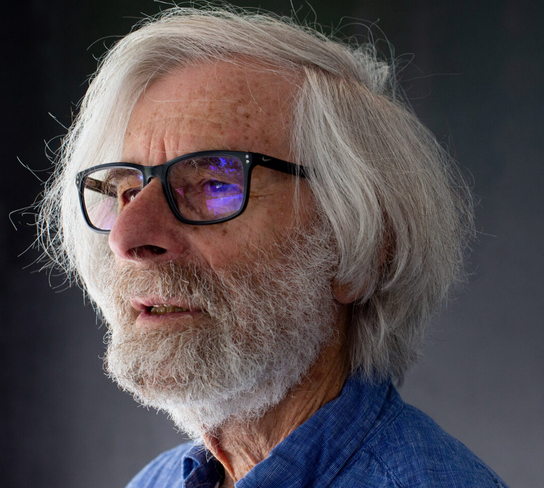
\includegraphics[width=\textwidth]{figs/Lamport}
               \caption{Leslie Lamport}
               \label{fig:grid_bl}
          \end{minipage}
          \hspace{1cm}  % Fixed spacing instead of \hfill
          \begin{minipage}{0.2\textwidth}
               \centering
               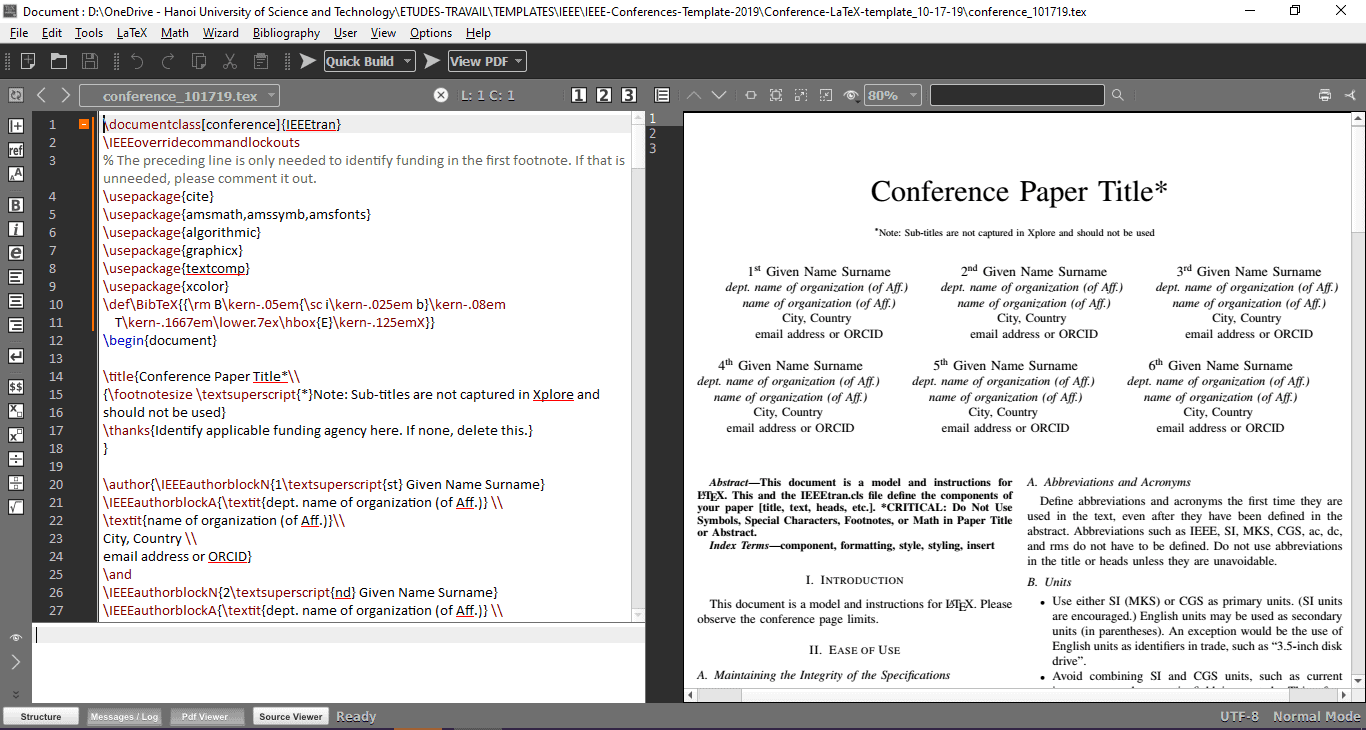
\includegraphics[width=\textwidth]{figs/latex_code}
               \caption{LaTeX Code Example}
               \label{fig:grid_br}
          \end{minipage}
     \end{figure}
     
     \begin{center}
          A 2×2 grid showing key elements of the LaTeX ecosystem
     \end{center}
\end{frame}
\begin{frame}[fragile]{Overlaying and Positioning Figures with TikZ}
     \textbf{TikZ for precise image overlays:}
     \begin{lstlisting}
          % Simple figure overlay using TikZ
          \begin{figure}
               \centering
               \begin{tikzpicture}
                    % Base image
                    \node[anchor=south west,inner sep=0] (image) at (0,0) {
                         \includegraphics[width=0.8\textwidth]{base_image}
                    };
                    
                    % Get the size of the image
                    \begin{scope}[x={(image.south east)},y={(image.north west)}]
                         % Overlay a smaller image (inset)
                         \node at (0.75,0.8) {
                              \includegraphics[width=0.3\textwidth]{small_image}
                         };
                         
                         % Add an arrow pointing to a feature
                         \draw[->,red,thick] (0.5,0.5) -- (0.7,0.7);
                         
                         % Add text label
                         \node[draw,fill=white] at (0.3,0.2) {Important feature};
                    \end{scope}
               \end{tikzpicture}
               \caption{Image with overlay elements}
               \label{fig:overlay}
          \end{figure}
     \end{lstlisting}
     
     \textbf{Benefits of TikZ approach:}
     \begin{itemize}
          \item Precise control over element positioning
          \item Can add arrows, text boxes, and other annotations
          \item Relative coordinates make resizing easier
          \item Great for highlighting specific features
     \end{itemize}
\end{frame}

\begin{frame}{Template: Figure with Overlays and Annotations}
     \begin{figure}
          \centering
          \begin{tikzpicture}
               % Base image
               \node[anchor=south west,inner sep=0] (image) at (0,0) {
                    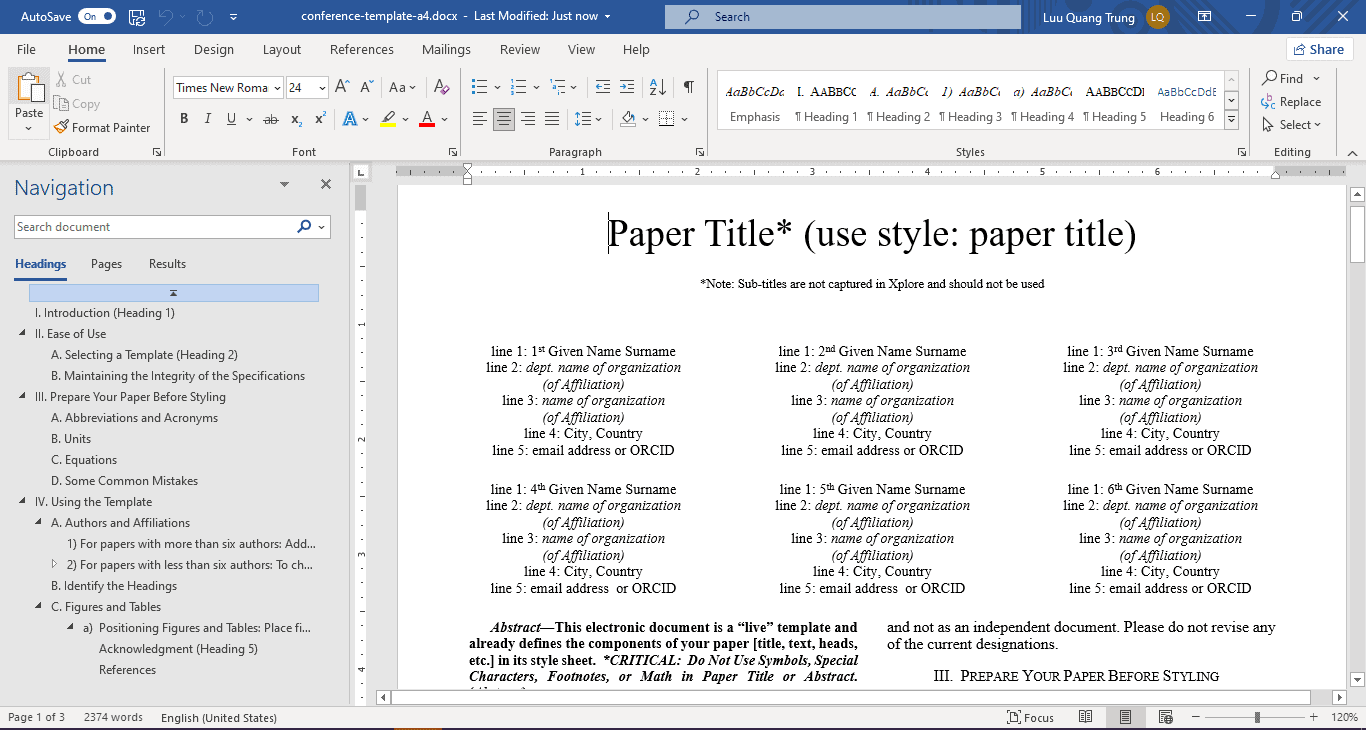
\includegraphics[width=0.9\textwidth]{figs/latex_code1}
               };
               
               % Get the size of the image
               \begin{scope}[x={(image.south east)},y={(image.north west)}]
                    % Overlay a smaller image
                    \node at (0.75,0.75) {
                         
\includegraphics[width=0.25\textwidth]{figs/latex_logo}
                    };
                    
                    % Add arrows and annotations
                    \draw[->,red,thick] (0.3,0.4) -- (0.45,0.4);
                    \node[draw,fill=white,font=\footnotesize] at (0.2,0.4) {This is};
                    
                    \draw[->,blue,thick] (0.6,0.2) -- (0.7,0.3);
                    \node[draw,fill=white,font=\footnotesize] at (0.5,0.15) {And this};
               \end{scope}
          \end{tikzpicture}
          \caption{Annotated LaTeX document structure}
          \label{fig:annotated}
     \end{figure}
     
     \begin{center}
          Using TikZ to create an annotated figure with inset and pointers
     \end{center}
\end{frame}

\begin{frame}[fragile]{Text Wrapping Around Figures}
     \textbf{Text wrapping using the wrapfig package:}
     \begin{lstlisting}
          % In preamble
          \usepackage{wrapfig}
          
          % Wrapping text around a figure
          \begin{wrapfigure}{r}{0.5\textwidth}
               \centering
               \includegraphics[width=0.45\textwidth]{image}
               \caption{Text wraps around this figure}
               \label{fig:wrapfig}
          \end{wrapfigure}
          
          This text will wrap around the figure on the right.
          The text continues flowing around the figure
          until enough lines have been typeset to
          match the height of the figure.
     \end{lstlisting}
     
     \textbf{wrapfig options:}
     \begin{itemize}
          \item First parameter: position (r, l, i, o for right, left, inside, outside)
          \item Second parameter: width of the figure space
          \item Works well with paragraphs of text
          \item Avoid using near section headings, lists, or other complex elements
          \item Add \texttt{\textbackslash usepackage\{wrapfig\}} to your preamble
     \end{itemize}
\end{frame}

\begin{frame}{Exercise: Advanced Figure Arrangements}
     \begin{practice}
          \textbf{Create a document with these figure arrangements:}
          \begin{enumerate}
               \item A side-by-side arrangement of two figures using minipage
               \item A 2×2 grid of figures with appropriate captions
               \item A main figure with annotations (arrows and text) using TikZ
               \item Text wrapping around a figure (requires wrapfig package)
          \end{enumerate}
     \end{practice}
     
     \textbf{Tips for success:}
     \begin{itemize}
          \item Start with simple layouts before combining techniques
          \item Use consistent sizing conventions (e.g., always as percentage of \texttt{\textbackslash textwidth})
          \item Remember to add all necessary packages in the preamble
          \item Test complex figures on a separate minimal document first
     \end{itemize}
     
     \begin{warning}
          Complex figure arrangements may require multiple compilation runs to display correctly
     \end{warning}
\end{frame}